\subsection{DUNE}
{{\footnotesize
\noindent Applying real-time ML methods to time-series data from DUNE detectors, exploring trigger-level anomaly detection and event selection with low latency constraints.


\begin{description}[labelwidth=4cm, labelsep=1em, leftmargin=4cm, itemsep=0.1em, parsep=0em]
  \item[date:] 2024-10-15
  \item[version:] v1.0
  \item[last\_updated:] 2024-10
  \item[expired:] unknown
  \item[valid:] yes
  \item[valid\_date:] 2024-10-15
  \item[url:] \href{https://indico.fnal.gov/event/66520/contributions/301423/attachments/182439/250508/fast\_ml\_dunedaq\_sonic\_10\_15\_24.pdf}{https://indico.fnal.gov/event/66520/contributions/301423/attachments/182439/250508/fast\_ml\_dunedaq\_sonic\_10\_15\_24.pdf}
  \item[doi:] 10.48550/arXiv.2103.13910
  \item[domain:]
    - High Energy Physics
  \item[focus:] Real-time ML for DUNE DAQ time-series data
  \item[keywords:]
    - DUNE
    - time-series
    - real-time
    - trigger
  \item[licensing:] Via Fermilab
  \item[task\_types:]
    - Trigger selection
    - Time-series anomaly detection
  \item[ai\_capability\_measured:]
    - Low-latency event detection
  \item[metrics:]
    - Detection efficiency
    - Latency
  \item[models:]
    - CNN
    - LSTM (planned)
  \item[ml\_motif:]
    - Anomaly Detection
  \item[type:] Benchmark (in progress)
  \item[ml\_task:]
    - Supervised Learning
  \item[solutions:] Solution details are described in the referenced paper or repository.
  \item[notes:] Prototype models demonstrated on SONIC platform

  \item[contact.name:] Andrew J. Morgan
  \item[contact.email:] unknown
  \item[datasets.links.name:] DUNE SONIC data
  \item[results.links.name:] ChatGPT LLM
  \item[fair.reproducible:] no
  \item[fair.benchmark\_ready:] No
  \item[id:] dune
  \item[Citations:] \cite{abud2021deep}
\end{description}

{\bf Ratings:} ~ \\

\begin{tabular}{p{0.15\textwidth} p{0.07\textwidth} p{0.7\textwidth}}
\hline
Rating & Value & Reason \\
\hline
dataset & 3 & Dataset lacks a public URL; FAIR metadata and versioning are missing
 \\
documentation & 3 & Documentation exists only in slides/GDocs; no implementation guide or structured release
 \\
metrics & 4 & Metrics are relevant but no benchmark baseline or detailed evaluation guidance is provided
 \\
reference\_solution & 2 & Autoencoder prototype exists but is not reproducible; RL model still in development
 \\
software & 1 & Code not available; no containerization or setup provided
 \\
specification & 4 & Constraints like latency thresholds are described qualitatively but not numerically defined
 \\
\hline
\end{tabular}

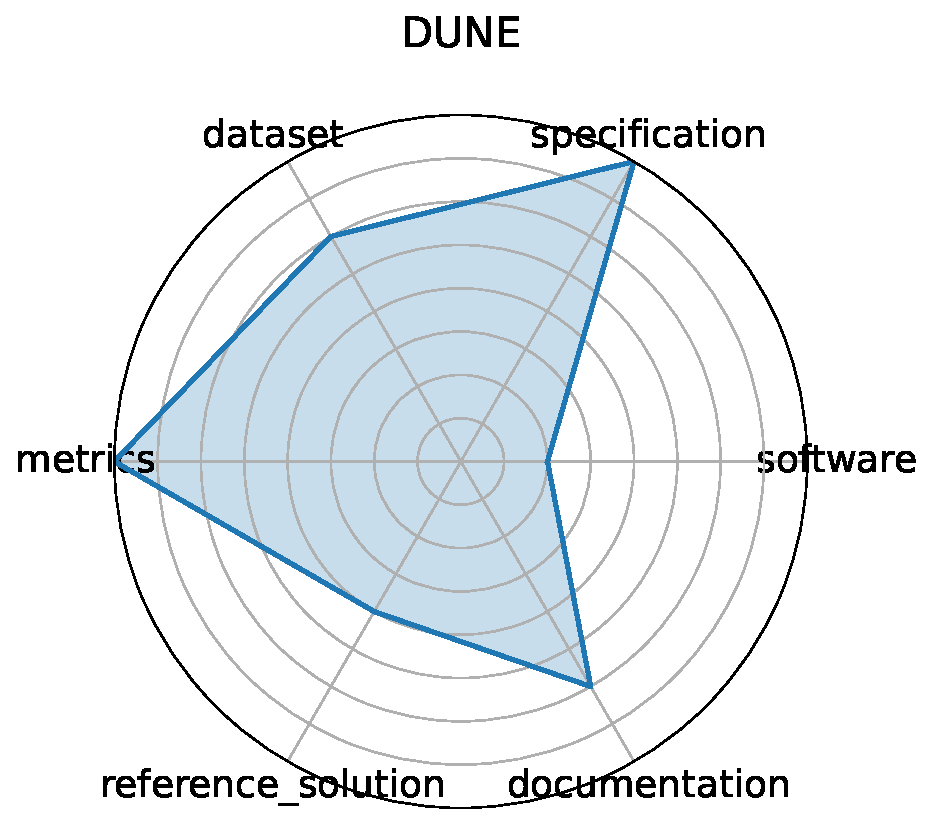
\includegraphics[width=0.2\textwidth]{dune_radar.pdf}
}}
\clearpage